General structure and tasks of an early detection system were already described in chapter \ref{early_detection_system}.
As it was mentioned before, an early detection system consists of two different components:

\begin{enumerate} 
    \item Several small embedded devices, deployed in the field. 
        They capture images with thermal camera, process them and send results over wireless network.
    \item One gateway, which is receiving results, and relays them to an application server over internet connection.
\end{enumerate} 

In this chapter we focus on the structure and design of deployed embedded system,both from hardware and firmware point of perspective.
We also describe construction of an application server, how received data is processed, stored and presented.

The general block diagram of an embedded system with a thermal camera is presented on the Figure \ref{system_diagram} 

\begin{figure}[ht]
        \centering
        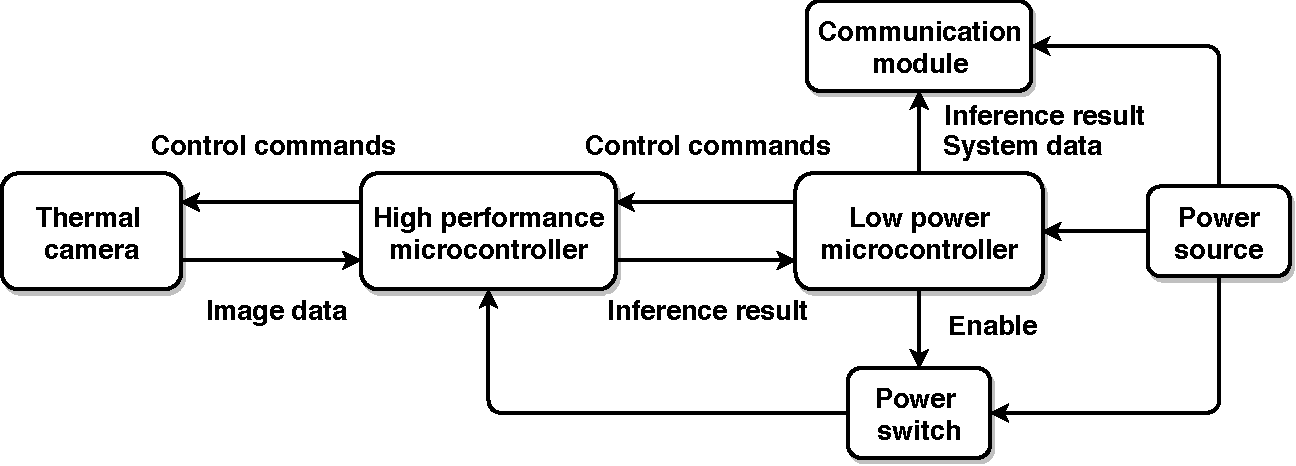
\includegraphics[width=1.0\linewidth]{system_diagram.pdf} 
        \caption{ General block diagram of an embedded system}
        \label{system_diagram}
\end{figure}

Embedded system will consist of two different microcontrollers with two distinct tasks, a thermal camera, PIR sensor, wireless communication module, power switch and battery.

Powerful, high performance microcontroller and thermal camera are turned off, to conserve battery life.
A less capable, but low power microcontroller will spend most the time in sleep, waiting for a trigger from PIR sensor.
PIR sensor will point in the same direction as the thermal camera and will detect any IR radiation of a passing object.

If an object passes PIR's field of vision, it triggers it, which in consequently wakes up a low power microcontroller.
Microcontroller will then enable power supply to high performance microcontroller and thermal camera, and send a command request for image capture and processing.

Thermal camera only communicates with high performance microcontroller, which configures it and requests image data.
That data is then inputted into neural network algorithm and an probability results are then returned to a low power microcontroller.
low power microcontroller then packs the data and sends it over radio through wireless communication module.
Power source to high performance microcontroller and thermal camera is then turned of to conserve power.
Diagram of described procedure can also be seen on Figure \ref{system_flow}.

\begin{figure}[ht]
        \centering
        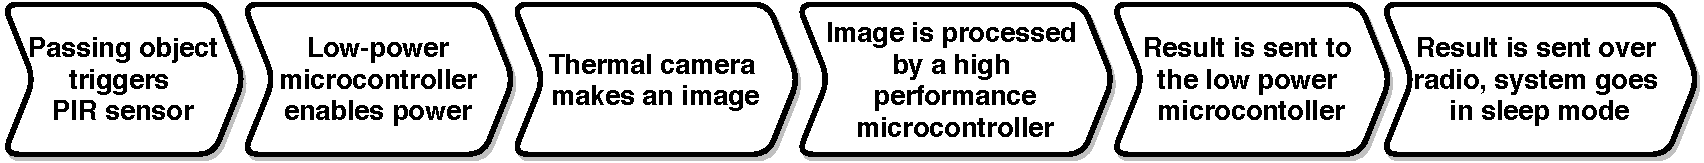
\includegraphics[width=1.0\linewidth]{system_flow.pdf} 
        \caption{ Diagram describing behavior of embedded early detection system} 
        \label{system_flow}
\end{figure}


\section{ Hardware}

In this section we present concrete components that we used to implement the embedded part of the early detection system.
Hardware version of embedded system diagram is presented on the Figure \ref{hardware_diagram}.
It should be noted that we did not include specific power source into the diagram.
Wisent Edge tracker board is general enough to work with different power sources, such as non-chargeable or chargeable batteries and or solar cells.

\begin{figure}[ht]
        \centering
        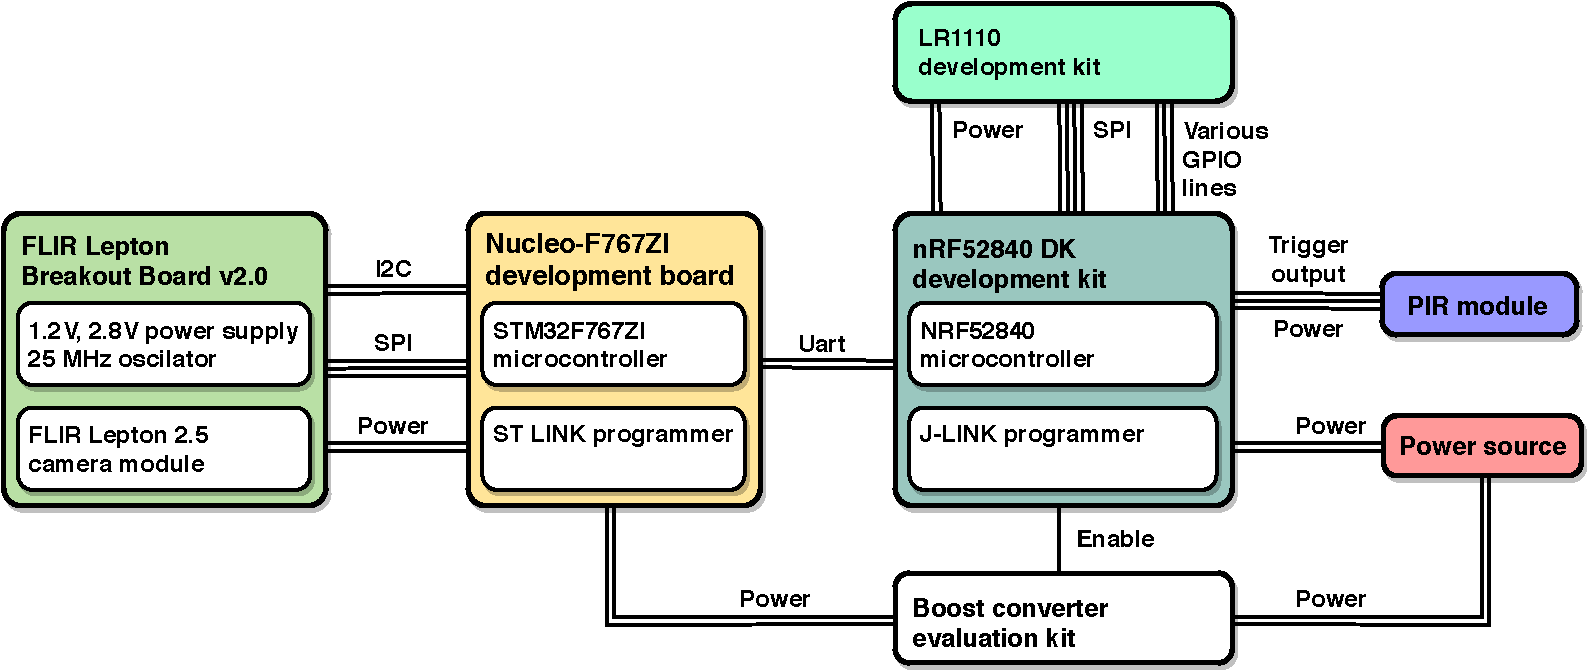
\includegraphics[width=1.0\linewidth]{hardware_diagram.pdf} 
        \caption{ Hardware diagram of embedded early detection system} 
        \label{hardware_diagram}
\end{figure}

\subsection{ Nucleo-F767ZI}

Nucleo-F767ZI (seen on Figure \ref{nucleo}) is a development board made by STMicroelectronics.
Board features STM32F767ZI microcontroller which has 2 \si{\mega\byte} of flash, 512 \si{\kilo\byte} of SRAM and can operate at clock speed of 216 \si{\mega\hertz}.
It also features different memory caches and flash accelerator, which provide extra boost in performance.
It is convenient to program it, as it includes on board ST-LINK programmer circuit.

We chose this microcontroller simply because it is one of more powerful general purpose microcontrollers on the market.
As we knew that neural networks are computationally expensive to compute and that models can be quite large in terms of memory, we selected it knowing that we can always scale down, if we have to.

\begin{figure}[ht]
        \centering
        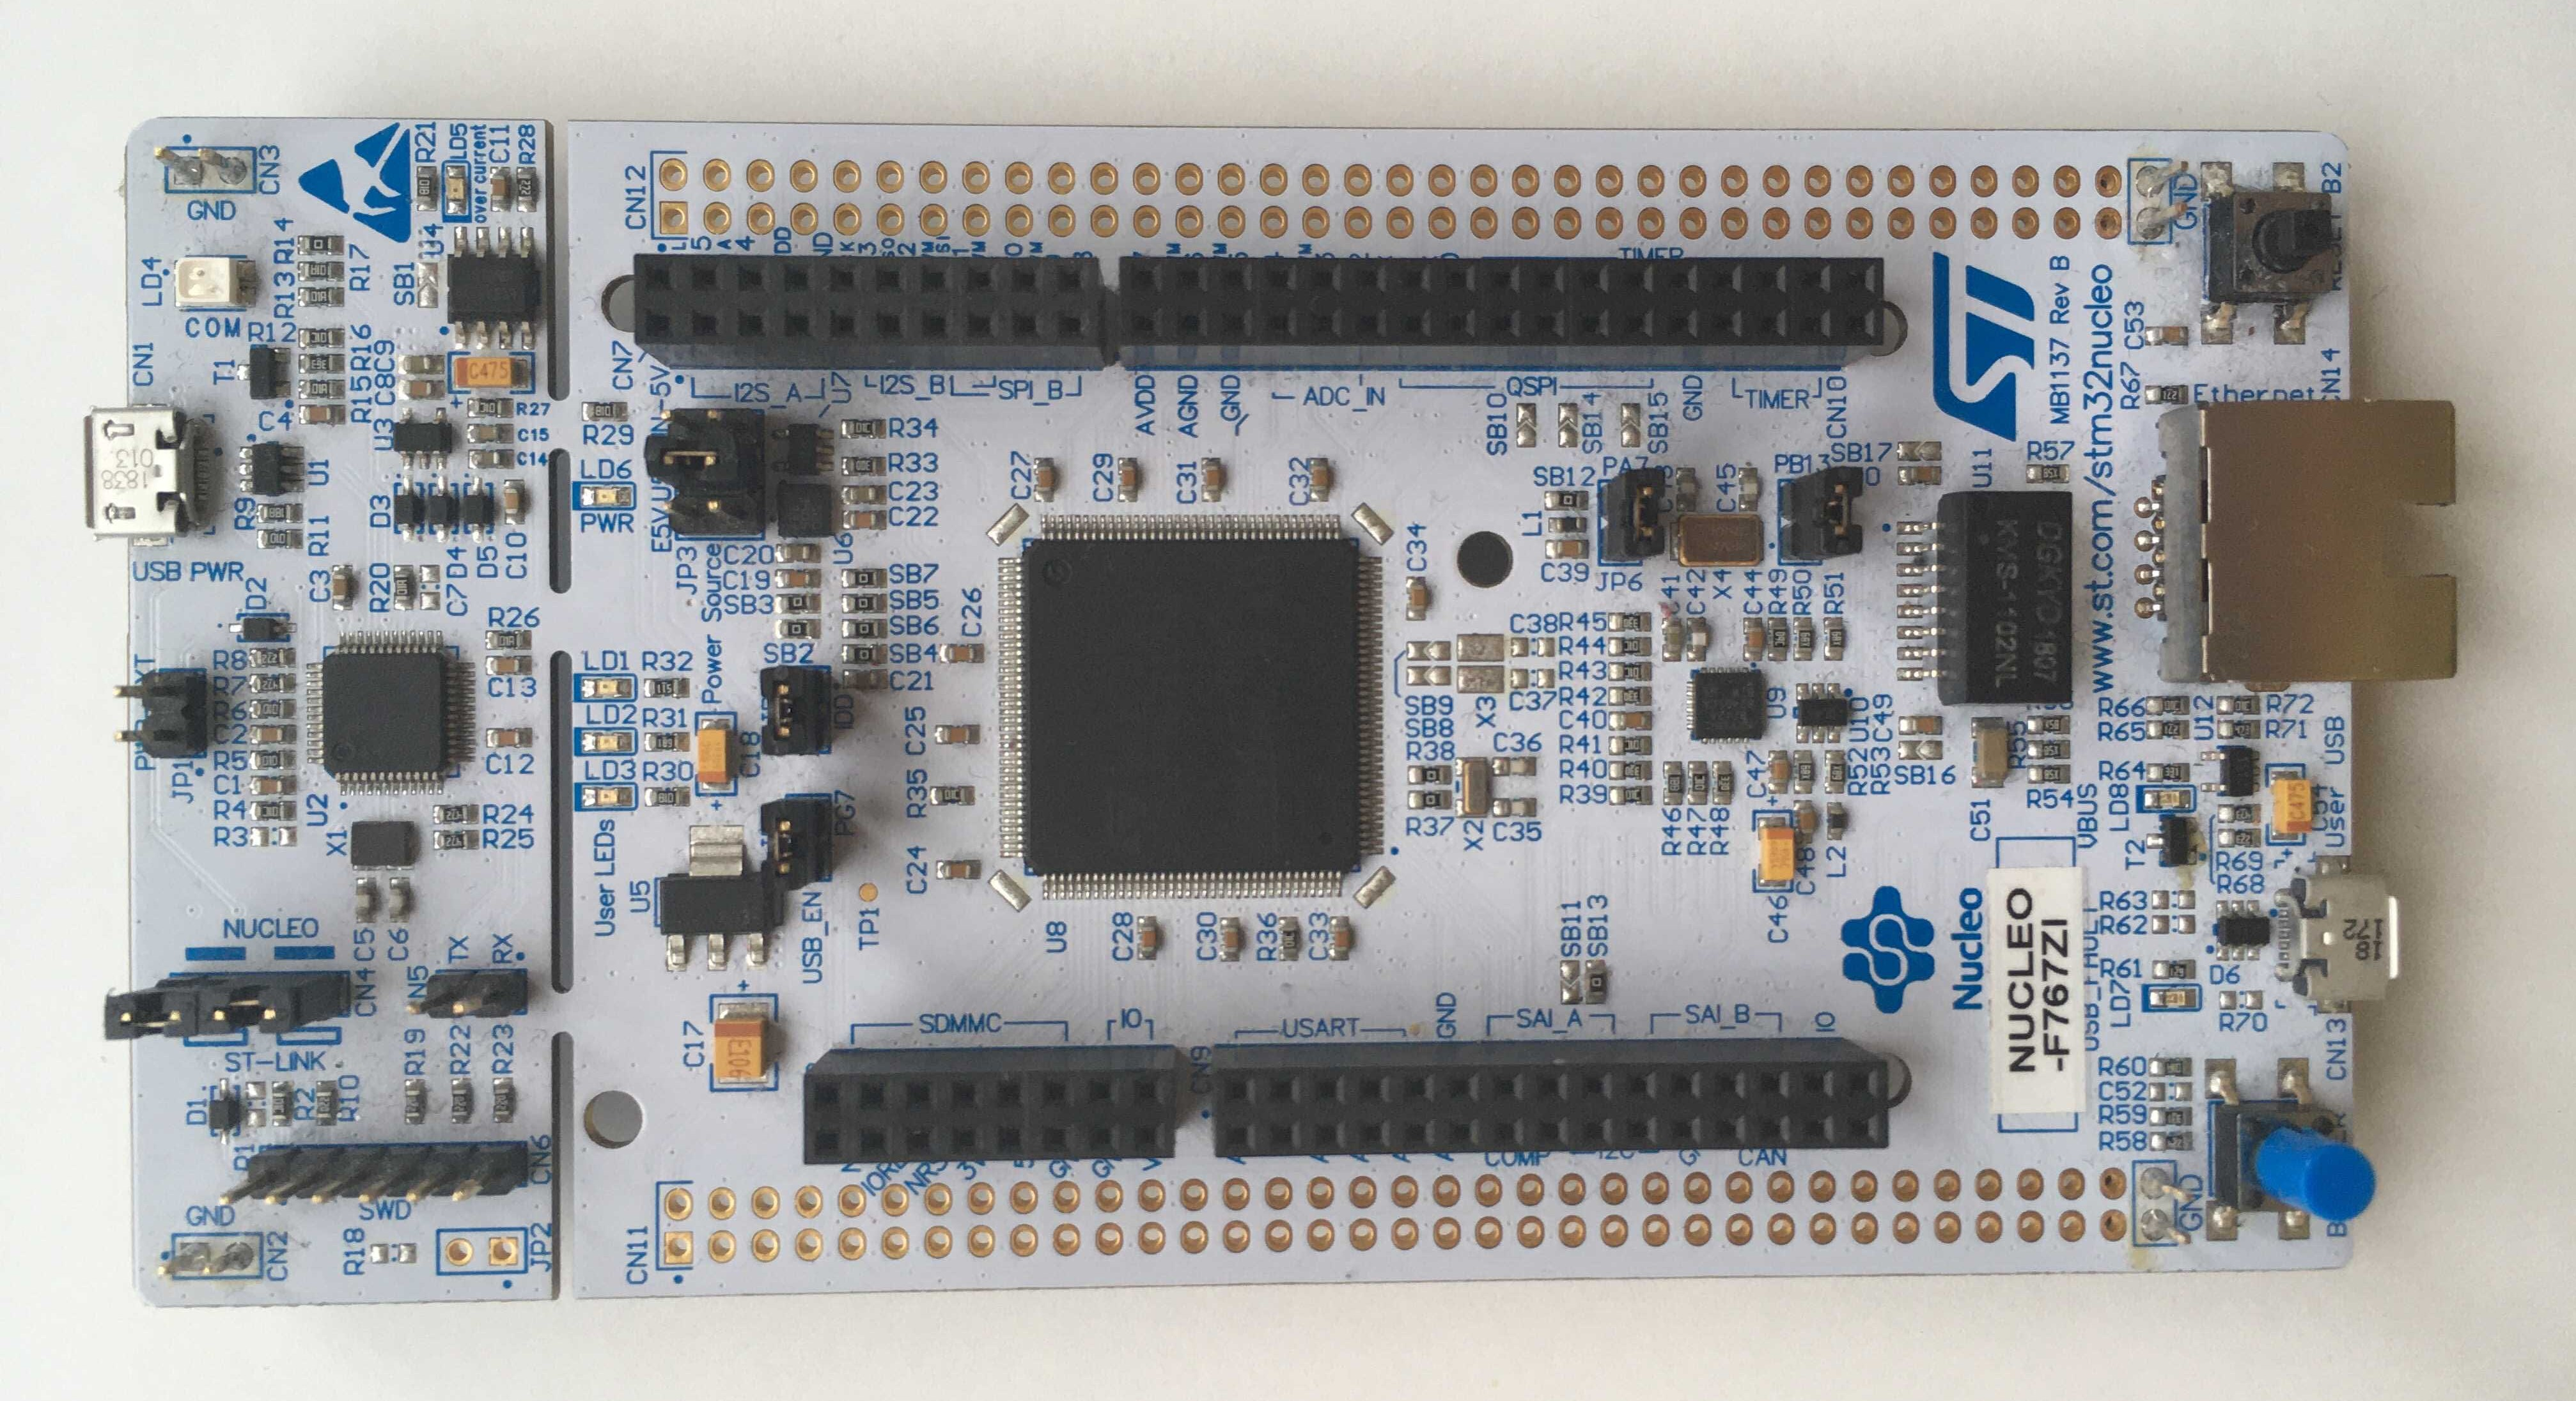
\includegraphics[height= 8cm]{nucleo.jpg} 
        \caption{ Nucleo-F767ZI development board} 
        \label{nucleo}
\end{figure}


\subsection{ Wisent Edge tracker}

%        WISENT BOARD,IRNASOV PRODUKT PREDSTAVI , SMART PARKS OPEN COLLARJK

    block diagram
An advanced sensor solution to conserve endangered wildlife and efficiently manage large park areas. OpenCollar is a conservation collaboration to design, support and deploy open-source tracking collar hardware and software for environmental and wildlife monitoring projects. The design of the tracking system is completely modular and it is possible to combine the modules into several different configurations, depending on the use case.

The Wisent Tracker features a medium sized waterproof housing, GPS tracker with LoRaWAN connectivity and years of battery life under normal conditions. The tracker is mounted to an animal using a highly durable BioThane collar with an optional drop-off mechanism also available.





\subsection{ Flir Lepton 2.5 camera module and Lepton breakout board}

In section \ref{thermal_cameras} it was described what kinds of thermal cameras exist and how do they work, and in section \ref{choosing_thermal} it was described why FLIR Lepton 2.5 was chosen.
However, not much was said about what sort of support circuitry FLIR camera needs and how do we actually make images with it.

FLIR Lepton camera needs to be powered from two different sources, 1.2 \si{\volt} and 2.8 \si{\volt}, as well it needs a reference clock of 25 \si{\mega\hertz}.
All of this is provided by Lepton breakout board, which can be seen on the Figure \ref{lepton_breakout}.
Front side of the breakout board contains a FLIR module socket and back side has two voltage regulators and a oscillator.
Breakout board can be powered from 3.3 to 5 \si{\volt} and also conveniently breaks out all communication pins in form of headers.

\begin{figure}[ht] 
    \begin{subfigure}[b]{0.5\textwidth}
        \centering
        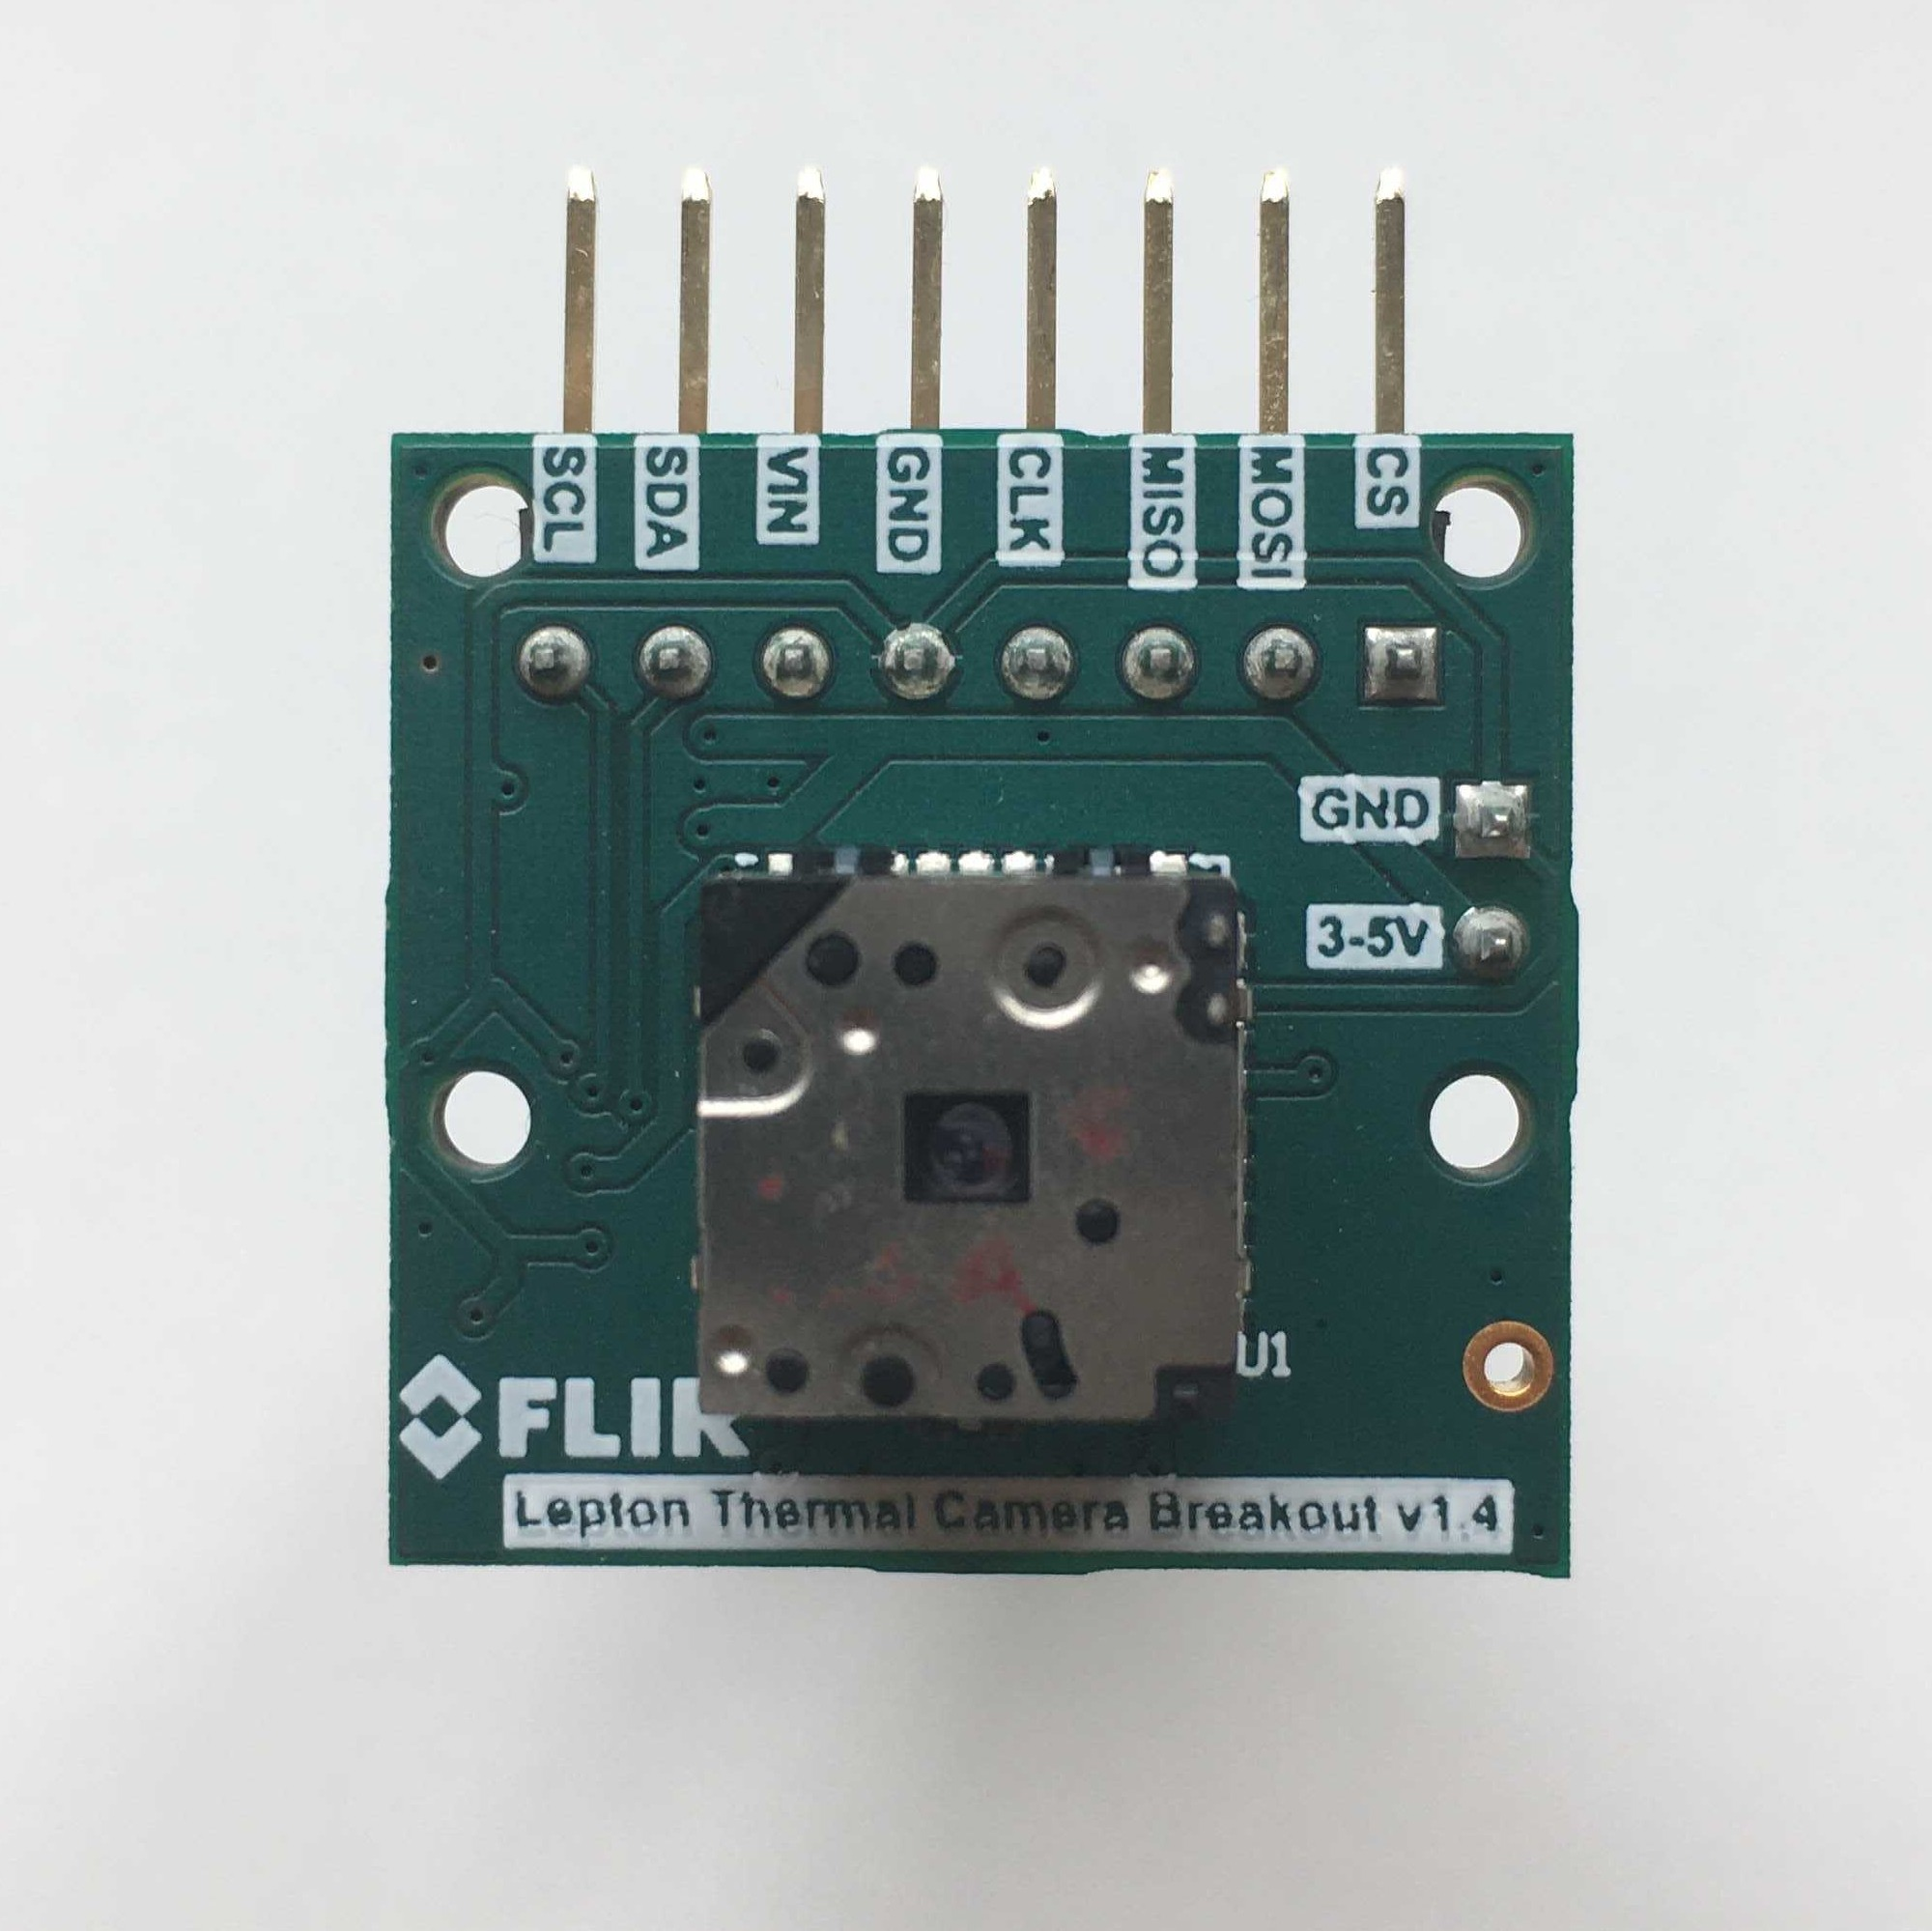
\includegraphics[width=1.0\linewidth]{flir_module_front.jpg} 
    \end{subfigure}
    \begin{subfigure}[b]{0.5\textwidth}
        \centering
        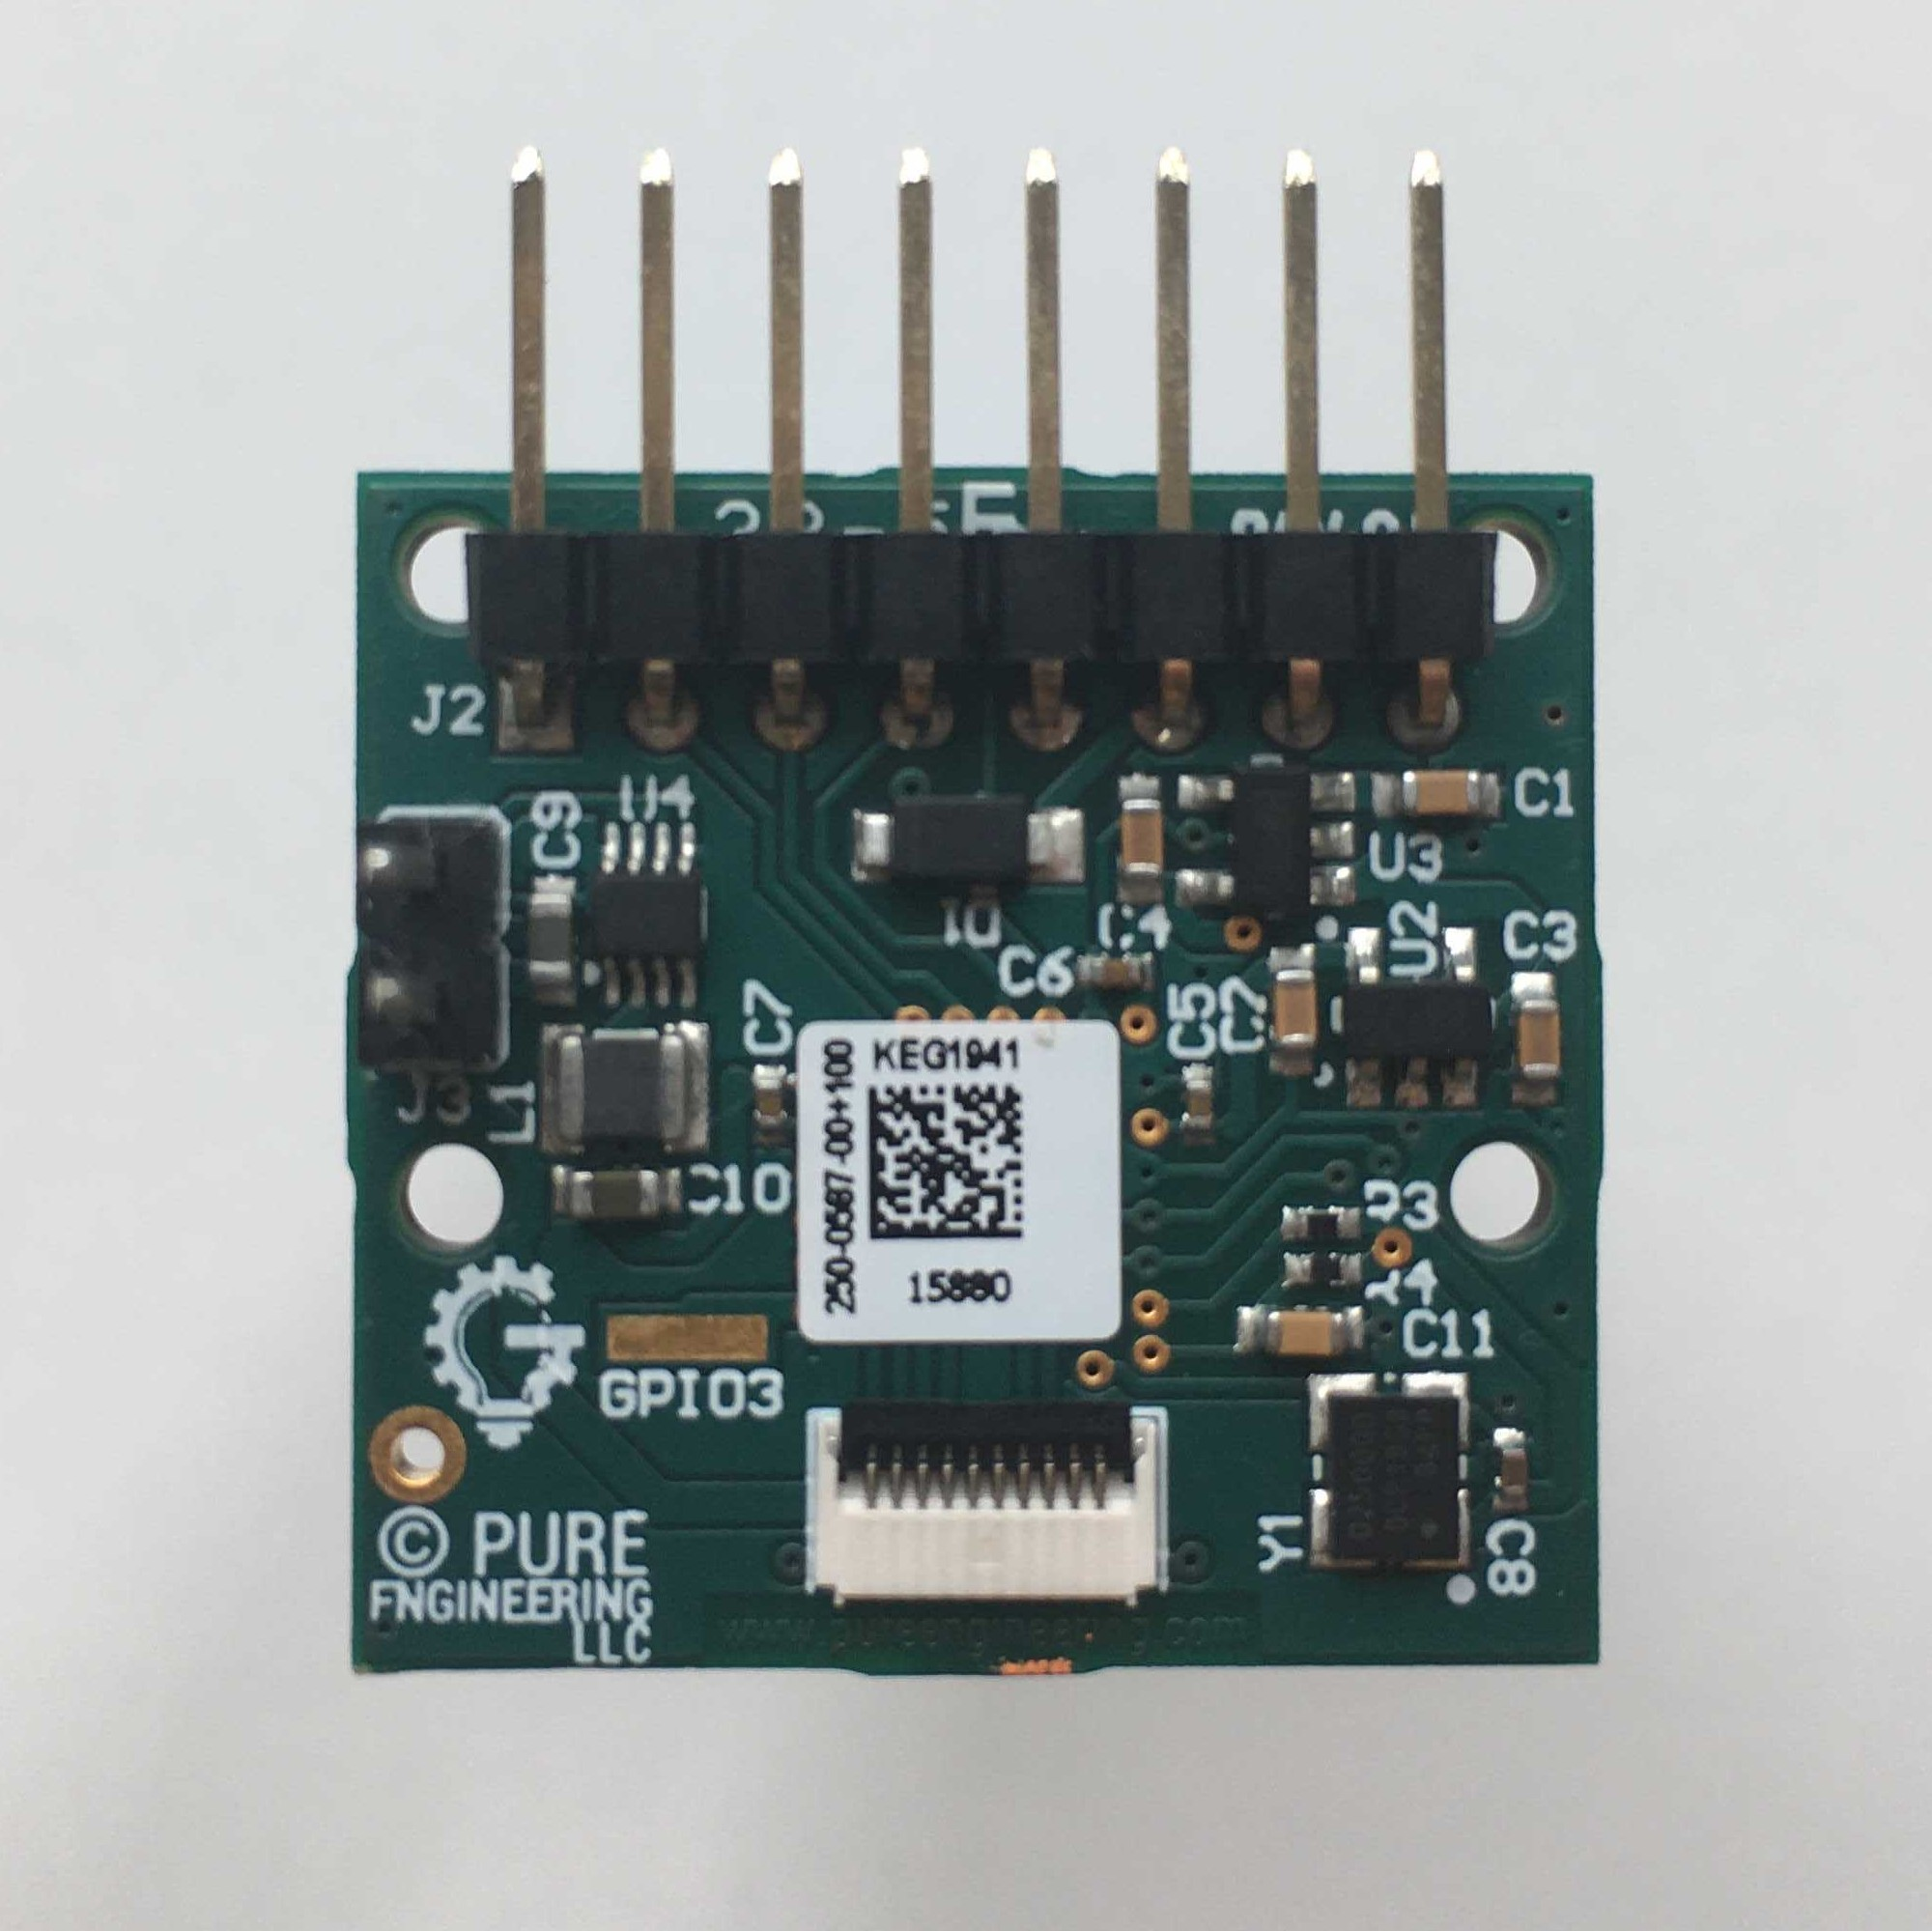
\includegraphics[width=1.0\linewidth]{flir_module_back.jpg} 
    \end{subfigure}
    \caption{ SOmethgn}
    \label{lepton_breakout}
\end{figure}

FLIR Lepton module itself conatins five different subsystems that work together and can be configured:

\begin{itemize}
    \item AGC – Automatic Gain Control, affects image contrast and quality
    \item SYS – System information
    \item VID – Video processing control
    \item OEM – Camera configuration for OEM customers
    \item RAD – Radiometry
\end{itemize}

AGC subsystem deals with converting a dynamic range of an IR sensor into a compact range that is more suitable for storing and displaying images.
In case of FLIR Lepton this is a 14-bit to 8-bit conversion.
For our purposes AGC subsystem was turned on, as the input to our neural network were 8-bit values.

Microcontroller communicates with FLIR camera over two interfaces: two wire interface (TWI) is used for sending commands and controlling the FLIR camera and Lepton's VoSPI protocol is used for image transfer.

TWI is a variation of an I2C protocol, instead of 8 bits, all transfers are 16 bits.
Internal structure of Lepton's control block can be seen on the Figure \ref{flir_lepton_cci}.
Whenever we are communicating with FLIR camera we have to specify which subsystem are we addressing, what type of action we want to do (get, set or run), length of data and data itself.

\begin{figure}[ht]
        \centering
        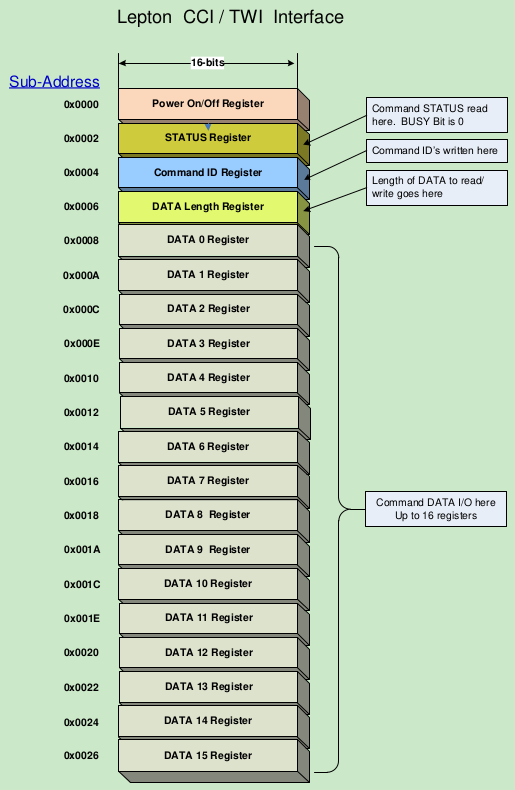
\includegraphics[height=10cm]{flir_lepton_cci.png} 
        \caption{ Command and control interface of FLIR Lepton camera.} 
        \label{flir_lepton_cci}
\end{figure}

Lepton's VoSPI protocol is used only to stream image data from camera module to the microcontroller, which means that MOSI line is not used.
Each image is fits into one VoSPI frame and each frame consists of 60 VoSPI packets.
One VoSPI packet contains an 2 bytes of an ID field, 2 bytes of an CRC field and 160 bytes of data\footnotemark, that represents one image line.

Refresh rate of VoSPI frames is 27 \si{\hertz}, however only every third frame is unique from the last one.
It is a job of the microcontroller to control the SPI clock speed and process each frame fast enough so that next unique frame is not discarded.

\footnotetext{ Because images pixel values fit into 14-bit range by default, it means that one pixel value needs two bytes of data (two most significant bytes are zero). That means that each image line (80 pixels) is stored into 160 bytes. If AGC coversion is turned on, each pixel is then mapped into 8-bit range, however the size of one line in VoSPI packet still remains 160 bytes, 8 most significant bits are simply zeros.}


\subsection{ PIR Sensor}

\section{ Firmware}
    arhitecture diagram 

\subsection{ Tools and development environment}
    libopencm3, 
    What tools you used, vim, openocd, Make, arm-none-eabi-gcc
    printf library
    wisent runs zephyr

\subsection{ Build system for TensorFlow Lite}
    Why you created it, 
    what problems does it solve that using tensorflow introduced, 
    how does it work (makefiles), diagram
    problems that you had. 
    Generally you should follow your github page. 
    TEST SETUP FOR RUNNING INFERENCE ON A COMPUTER

\subsection{ Running inference on a microcontoller}
    explain how tensorflow works on a micro, interpreted approach vs boilerplate code. 

\subsection{ Wisent board control firmware}
    flow diagram
    cli interface (this should be put somewhere, or not?)





%\section{ Server side components/software}
%\subsection{ TTN}
%\subsection{ NODE-RED}
%\subsection{ InfluxDB}
%\subsection{ Grafana}
%
%
%
%
%
%
%
%
%
%
%
%
%Part of this thesis was concerned with porting TFLite Micro to \textbf{libopencm3}, our platform of choice.
%To compile source files and build binaries TFLite Micro uses build automation tool \textbf{GNU Make}.
%One large makefile that includes several platform specific makefiles dictates how firmware is built.
%By providing command line arguments users decide which example has to be compiled and for which platform.
%The build system makes some assumptions about locations of the platform specific files, which in case of example projects are scattered over GitHub repository.
%This and several other reasons make library hard to use when porting it to a new platform.
%In section TODO ADD REFERENCE we describe our build system that keeps library and application specific code separated in a clear and concise manner.
%
